\definecolor{shadecolor}{rgb}{0.9,0.9,0.9}
\allsectionsfont{\centering \normalfont\scshape}











\section{\textbf{While Loops}}

A {\color{red}while loop} statement in Python programming language repeatedly executes a target statement as long as a given condition is true.

\vspace{1cm}
The condition may be any expression, and true is any non-zero value. The loop iterates while the condition is true.When the condition becomes false, program control passes to the line immediately following the loop.In Python, all the statements indented by the same number of character spaces after a programming construct are considered to be part of a single block of code. Python uses indentation as its method of grouping statements.

\begin{marginfigure}
  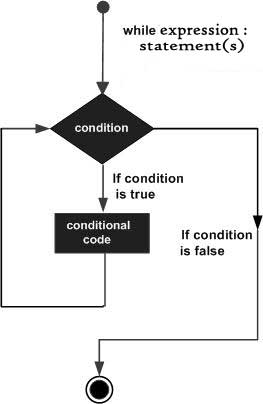
\includegraphics[width=\linewidth]{whileloop.png}
  \caption{Flow diagram about how the while loop works}
  \label{fig:marginfig}
\end{marginfigure}

\vspace{0.5cm}
\subsection{Python code example}
\begin{framed}
\begin{verbatim}

count = 0
while (count < 9):
   print 'The count is:', count
   count = count + 1

print "Good bye!"

\end{verbatim}
\end{framed}

\subsection{Output}
\marginnote[40pt]{The code will produce the following output.}
\begin{shaded}
\begin{verbatim}
>>> 
The count is: 0
The count is: 1
The count is: 2
The count is: 3
The count is: 4
The count is: 5
The count is: 6
The count is: 7
The count is: 8
Good bye!
>>> 
\end{verbatim}
\end{shaded}

\subsection{Infinite Loop}
A loop becomes {\color{red}infinite loop} if a condition never becomes {\textbf{FALSE}}. You must use caution when using while loops because of the possibility that this condition never resolves to a FALSE value. This results in a loop that never ends. Such a loop is called an infinite loop.

An infinite loop might be useful in client/server programming where the server needs to run continuously so that client programs can communicate with it as and when required.
\marginnote[40pt]{This python code is an example of how infinite loop can be created.}
\begin{framed}
\begin{verbatim}
var = 1
while var == 1:
   num = raw_input("Enter a number  :")
   print "You entered: ", num

print "Good bye!"
\end{verbatim}
\end{framed}

\marginnote[40pt]{This code creates an infinite loop where it will need your input of any number.Once you input any number, it will output it like if you input "X" it will show back "X".}
\begin{shaded}
\begin{verbatim}

Enter a number  :X
You entered:  x
Enter a number  :Y
You entered:  Y
Enter a number  :Z
You entered:  Z
Enter a number between :

\end{verbatim}
\end{shaded}

To break the loop you will either need to add the "{\color{red}break}" command in your code OR press {\textbf{CTRL+C} to exit the program.

\subsection{Using else statements with while loops}
Python supports to have an else statement associated with a loop statement.

If the {\color{red}else statement} is used with a while loop, the else statement is executed when the condition becomes false.

\vspace{1cm}







\begin{framed}
\begin{verbatim}

count = 0
while count < 5:
   print count, " is  less than 5"
   count = count + 1
else:
   print count, " is not less than 5"

\end{verbatim}
\end{framed}

\marginnote[-140pt]{The following code illustrates the combination of an else statement with a while statement that prints a number as long as it is less than 5, otherwise else statement gets executed.}

\marginnote[40pt]{This is the output in python when the code above is executed.}
\begin{shaded}
\begin{verbatim}
>>> 
0 is less than 5
1 is less than 5
2 is less than 5
3 is less than 5
4 is less than 5
5 is not less than 5
>>> 
\end{verbatim}
\end{shaded}





